\documentclass[twoside,10pt]{article}
%=================================================
% Basics
%=================================================
\usepackage{fixltx2e} % Makes \( \) equation style robust, among other
                      % things. Must be the first package.


% Makes ligatured fonts searchable and copyable in pdf readers
\usepackage{cmap} % Load before fontenc 

% Always include these font encodings in your document 
% unless you have a very good reason.
\usepackage[T1]{fontenc}
\usepackage[utf8]{inputenc}

\usepackage{verbatim}

%=============
% Fonts
%=============

\usepackage{lmodern} % Improved version of computer modern
\usepackage[scale=0.88]{tgheros} % Helvetica clone for sans serif font


\newcommand\hmmax{2} % Default is 3.
\newcommand\bmmax{2} % Default is 4.

\usepackage{bm} % boldmath must be called after the package
\providecommand{\mathbold}[1]{\bm{#1}}

%=============
% AMS Packages and fonts
%=============
\usepackage{amsmath,amsbsy,amsgen,amscd,amsthm,amsfonts,amssymb} 

%=============
% Margins and paper size
%=============
\usepackage[centering,top=1.5in,bottom=1.2in,left=1.4in,right=1.4in]{geometry}
\usepackage{parskip}


%=============
% Section headings
%=============
\usepackage[sf,bf,compact]{titlesec}

%=============
% Tables and lists
%=============
\usepackage{booktabs,longtable,tabu} % Nice tables
\setlength{\tabulinesep}{1mm}
\usepackage[font=small,margin=10pt,labelfont={sf,bf},labelsep={space}]{caption}

%=============
% Code output
%=============
% \usepackage{listings}
% \usepackage{minted}




\usepackage{enumitem}
\setitemize{itemsep=0pt} 
\setenumerate{itemsep=0pt}
\setlist{labelindent=\parindent,%  % Recommended by enumitem package
  font=\sffamily}


%=============
% Hyperlink colors
%=============
\usepackage[usenames,dvipsnames]{xcolor}
\definecolor{steelblue}{HTML}{A1BDC7}
\definecolor{orange}{HTML}{D98C21}
\definecolor{silver}{HTML}{B0ABA8}
\definecolor{rust}{HTML}{B8420F}
\definecolor{seagreen}{HTML}{2E6B69}
\definecolor{joshua}{HTML}{FBDC7F}
\definecolor{darksky}{HTML}{154c79}

\colorlet{steelblue}{silver!30!white}
\colorlet{darkorange}{orange!85!black}
\colorlet{darksilver}{silver!85!black}
\colorlet{darksteelblue}{steelblue!85!black}
\colorlet{darkrust}{rust!85!black}
\colorlet{darkseagreen}{seagreen!85!black}

\usepackage{url}
\usepackage[colorlinks=true]{hyperref}
\hypersetup{linkcolor=darkrust}    
\hypersetup{citecolor=darkseagreen}      
\hypersetup{urlcolor=darksilver}     

%=============
% Microtype
%=============
\usepackage[final]{microtype} 

%=====================
% Header
%=====================
% \usepackage{fancyhdr}
% \usepackage{nopageno} % Gets rid of page number at the bottom
% \fancyhf{} % Clear header style
% \renewcommand{\headrulewidth}{0.5pt} % remove the header rule
% \pagestyle{fancy}
% \fancyhead[LE,RO]{\textsf{\small \thepage}}
% 
% \setlength{\headheight}{14pt}
%=====================
% Fix delimiters
%=====================

% Fixes \left and \right spacing issues. See discussion at
% http://tex.stackexchange.com/questions/2607/spacing-around-left-and-right
\let\originalleft\left
\let\originalright\right
\renewcommand{\left}{\mathopen{}\mathclose\bgroup\originalleft}
\renewcommand{\right}{\aftergroup\egroup\originalright}

%=================================================
% Math macros
%=================================================

%=============
% Generalities
%=============
\usepackage{mathtools}
\mathtoolsset{centercolon}  % Makes := typeset correctly for definitions

%%% Equation numbering
%\numberwithin{equation}{section} 

%%% Annotations
\newcommand{\notate}[1]{\textcolor{red}{\textbf{[#1]}}}

%==============
% Symbols
%==============
\let\oldphi\phi
\let\oldeps\epsilon

\renewcommand{\phi}{\varphi}
\renewcommand{\epsilon}{\varepsilon}
\newcommand{\eps}{\varepsilon}

%==============
% Constants
%==============

% Set constants upright
\newcommand{\cnst}[1]{\mathrm{#1}}  
\newcommand{\econst}{\mathrm{e}}

\newcommand{\zerovct}{\vct{0}} % Zero vector
\newcommand{\Id}{\mathbf{I}} % Identity matrix
\newcommand{\onemtx}{\bm{1}}
\newcommand{\zeromtx}{\bm{0}}

%==============
% Sets
%==============
\providecommand{\mathbbm}{\mathbb} % In case we don't load bbm

% Reals, complex, naturals
\newcommand{\R}{\mathbbm{R}}
\newcommand{\C}{\mathbbm{C}}
\newcommand{\K}{\mathbbm{K}}
\newcommand{\N}{\mathbbm{N}}

%==============
% Probability
%==============
\newcommand{\Prob}{\operatorname{\mathbbm{P}}}
\newcommand{\Expect}{\operatorname{\mathbb{E}}}

%==============
% Vectors and matrices 
%==============
\newcommand{\vct}[1]{\mathbold{#1}}
\newcommand{\mtx}[1]{\mathbold{#1}}

\newcommand{\mrange}{\operatorname{range}}
\newcommand{\mnull}{\operatorname{null}}


\DeclareMathOperator*{\argmax}{argmax}
\DeclareMathOperator*{\argmin}{argmin}

\bibliographystyle{plain}

\begin{document}
\nocite{*}

\title{CSE 6643 Homework 3}
\author{Karl Hiner}
\date{}
\maketitle

\section{One-upping [25 pts]}
Let $\mtx{A} \in \R^{m \times m}$ have full rank. Assume that we have already computed the QR decomposition of $\mtx{A}$.
For $\mtx{u}, \mtx{v} \in \R^m$, we call the matrix $\mtx{B} = \mtx{A} + \mtx{u}\mtx{v}^{T}$ a rank-1 update of $\mtx{A}$. 

\subsection*{(a) [5 pts]}
Prove that if $\vct{v}^{T} \mtx{A}^{-1} \vct{u} \neq - 1$, then $\mtx{B}$ is invertible.

\quad Let $\vct{x} \in \R^{m}$ be a non-zero vector. Then,
\begin{align*}
  \vct{v}^{T} \mtx{A}^{-1} \vct{u} &\neq -1\\
  1 &\neq -\vct{v}^{T} \mtx{A}^{-1} \vct{u} \\
  \vct{v}^{T} \vct{x} &\neq -(\vct{v}^{T} \mtx{A}^{-1} \vct{u})(\vct{v}^{T} \vct{x}) \\
  \vct{x} &\neq -\mtx{A}^{-1} \mtx{u}(\vct{v}^{T} \vct{x}) \\
  \mtx{A} \vct{x} &\neq -\mtx{u}\vct{v}^{T} \vct{x} \\
  \left(\mtx{A} + \mtx{u}\vct{v}^{T}\right)\vct{x} &\neq \mtx{0}. \\
  \mtx{B}\vct{x} &\neq \vct{0}
\end{align*}

\quad Thus, if $\vct{v}^{T} \mtx{A}^{-1} \vct{u} \neq -1$, there are no nontrivial solutions for $\mtx{B}\vct{x} = \vct{0}$, and so $\mtx{B}$ is invertible.

\subsection*{(b) [10 pts]} 
Design an algorithm that provably solves the system of equations $\mtx{B} \mtx{x} = \mtx{b}$ in $O(m^2)$ operations. 
\begin{align*}
  \vct{x} &= \mtx{B}^{-1}\vct{b}&\text{(assume $\mtx{B}$ is invertible)}\\
  &= \left(\mtx{A} + \vct{u}\vct{v}^T\right)^{-1}\vct{b}&\text{(since $\mtx{B} = \mtx{A} + \vct{u}\vct{v}^T$)}\\
  &= \left(\mtx{A}^{-1} - \dfrac{\mtx{A}^{-1}\vct{u}\vct{v}^T\mtx{A}^{-1}}{1+\vct{v}^T\mtx{A}^{-1}\vct{u}}\right)\vct{b}&\text{(Sherman–Morrison formula \cite{sherman_adjustment_1950})}\\
  &= \mtx{A}^{-1}\vct{b} - \dfrac{\mtx{A}^{-1}\vct{u}\vct{v}^T}{1+\vct{v}^T\mtx{A}^{-1}\vct{u}}\mtx{A}^{-1}\vct{b}&\text{(note: (1a above), $\mtx{B}$ invertible $\implies$ den $\neq 0$)}\\
  &= \tilde{\vct{x}} - \dfrac{\tilde{\vct{u}}\vct{v}^T}{1+\vct{v}^T\tilde{\vct{u}}}\tilde{\vct{x}}&\text{(let $\tilde{\vct{x}} \equiv \mtx{A}^{-1}\vct{b}, \tilde{\vct{u}} \equiv \mtx{A}^{-1}\vct{u}$)}\\
  &= \left[\vct{I} + \left(\dfrac{-1}{1+\vct{v}^T\tilde{\vct{u}}}\right)\vct{\tilde{\vct{u}}\vct{v}^T}\right]\tilde{\vct{x}}&\text{(rearrange)}\\
  &= \left(\vct{I} + \alpha\tilde{\vct{u}}\vct{v}^T\right)\tilde{\vct{x}}&\text{(let $\alpha \equiv \dfrac{-1}{1+\vct{v}^T\tilde{\vct{u}}}$)}
\end{align*}
\quad Thus, we have derived an expression for $\vct{x}$ in terms of a scalar $\alpha$ and vectors $\tilde{\vct{u}}, \tilde{\vct{x}}$.

\quad Vectors $\tilde{\vct{u}}$ and $\tilde{\vct{x}}$ are both defined in terms of $\mtx{A}^{-1} = \mtx{R}^{-1}\mtx{Q}^T$, where we assume $\mtx{R}$ and $\mtx{Q}$ have already been computed.
Thus, both vectors can be computed using back substitution in $O(m^2)$.
$\alpha$ can then be computed in $O(m)$, and the final expression for $\vct{x}$ involves a vector-scalar product, a vector outer product, an identity addition, and a matrix-vector multiplication, for a total of
$$O(m) + O(m^2) + O(m) + O(m^2) = O(2m) + O(m^2) = O(m^2)$$
operations.

\quad Here is the algorithm:
\begin{enumerate}
  \item Solve $\mtx{R}\tilde{\vct{x}} = \mtx{Q}^T\vct{b}$ for $\tilde{\vct{x}}$ using back substitution. ($O(m^2)$)
  \item Solve $\mtx{R}\tilde{\vct{u}} = \mtx{Q}^T\vct{u}$ for $\tilde{\vct{u}}$ using back substitution. ($O(m^2)$)
  \item Compute the scalar $\alpha = \dfrac{-1}{1+\vct{v}^T\tilde{\vct{u}}}.$ ($O(m)$)
  \item Finally, compute the solution $\vct{x} = \left(\vct{I} + \left(\left(\alpha\tilde{\vct{u}}\right)\vct{v}^T\right)\right)\tilde{\vct{x}}.$ ($O(m^2)$)
\end{enumerate}

\quad Since the highest-order term across all steps is $O(m^2)$, the total number of operations is $O(m^2)$.

\subsection*{(c) r-upping [10 pts]}
Extend the algorithm from the previous exercise to the case of $\mtx{B} = \mtx{A} + \mtx{U}\mtx{V}^{T}$, for $\mtx{U},\mtx{V} \in \R^{m \times r}$ and $r \ll m$.
Calculate the asymptotic complexity of the resulting algorithm.

\quad The Sherman-Morrison formula was the key step above.
Here, we will use the generalization of that formula, the Woodbury matrix identity \cite{woodbury_1950}.
Given the definitions above, the Woodbury matrix identity states that if $\left(\mtx{I} + \mtx{V}^T\mtx{A}^{-1} \mtx{U}\right)$ is invertible,
$$\mtx{B}^{-1} = \mtx{A}^{-1} - \mtx{A}^{-1}\mtx{U} \left(\mtx{I} + \mtx{V}^T\mtx{A}^{-1}\mtx{U}\right)^{-1} \mtx{V}^T\mtx{A}^{-1}.$$
Thus, we can express the solution $\vct{x}$ as
\begin{align*}
  \vct{x} &= \left(\mtx{A}^{-1} - \mtx{A}^{-1}\mtx{U} \left(\mtx{I} + \mtx{V}^T\mtx{A}^{-1}\mtx{U}\right)^{-1} \mtx{V}^T\mtx{A}^{-1}\right)\vct{b}\\
  &= \mtx{A}^{-1}\vct{b} - \mtx{A}^{-1}\mtx{U} \left(\mtx{I} + \mtx{V}^T\mtx{A}^{-1}\mtx{U}\right)^{-1} \mtx{V}^T\mtx{A}^{-1}\vct{b}\\
  &= \tilde{\vct{x}} - \tilde{\mtx{U}} \left(\mtx{I} + \mtx{V}^T\tilde{\mtx{U}}\right)^{-1} \mtx{V}^T\tilde{\vct{x}} &\text{(let $\tilde{\vct{x}} \equiv \mtx{A}^{-1}\vct{b}, \tilde{\mtx{U}} \equiv \mtx{A}^{-1}\mtx{U}$)}\\
  &= \tilde{\vct{x}} - \tilde{\mtx{U}} \mtx{C}^{-1}\mtx{V}^T\tilde{\vct{x}} &\text{(let $\mtx{C} = \mtx{I} + \mtx{V}^T\tilde{\mtx{U}}$)}
\end{align*}
Note that, since $\tilde{\mtx{U}} \in \R^{m \times r}$, and $\mtx{V}^T \in \R^{r \times m}$, we can compute the matrix product $\tilde{\mtx{U}}\mtx{V}^T$ using $O(m^2r)$ operations.

\quad Here is the algorithm:
\begin{enumerate}
  \item Solve $\mtx{R}\tilde{\vct{x}} = \mtx{Q}^T\vct{b}$ for $\tilde{\vct{x}}$ using back substitution (same as step 1 in (b)). ($O(m^2)$)
  \item Compute $\tilde{\mtx{U}} = \mtx{A}^{-1}\mtx{U}$ by solving each of the linear systems $\mtx{R}\tilde{\vct{u}}_i = \mtx{Q}^T\vct{u}_i$ for $\tilde{\vct{u}}_i$, where $\tilde{\vct{u}}_i$ is the $i$th column of $\tilde{\mtx{U}}$ and $\vct{u}_i$ is the $i$th column of $\mtx{U}$.
  This can be done using back substitution (as in step 2 in (b)) for each of the $r$ columns. ($O(m^2r)$)
  \item \textit{I was unable to complete this.} I feel that this is very close. Finding $\mtx{C}^{-1}$ should be possible using another linear system, similarly in $O(m^2r)$ time, and I think it can be done in a way that actually avoids an expensive final computation step by the correct formulation of this linear system (ideally using only $O(mr)$ matrix-vector/vector-vector multiplications).
\end{enumerate}

This solution should be computable in $O(m^2r)$ time.

\section{You Factor [25 pts]}
In class we have seen that if $\tilde{\vct{x}} \in \R^{m}$ is the solution to the system $\mtx{A}\vct{x} = \vct{b}$, as computed by unpivoted LU factorization, we have  
\begin{equation}
  \left(\mtx{A} + \mtx{E}\right)\tilde{\vct{x}} = \vct{b}.  
\end{equation}
For $u$ the unit roundoff error and $\tilde{\mtx{L}}, \tilde{\mtx{U}}$ the LU factors computed in finite precision, we have
\begin{equation}
  \left|\mtx{E}\right| \leq m u \left(2 \left|\mtx{A}\right| + 4 \left|\tilde{\mtx{L}} \right| \left|\tilde{\mtx{U}}\right|\right) + O(u^2).
\end{equation}
Here, $|\cdot|$ signifies the element-wise absolute values and $\leq$ is interpreted element-wise, as well.
In this problem, we investigate the conclusions from this bound in the case of row-pivoted LU factorization.

\subsection*{(a) [7.5 pts]}
Deduce that under row-pivoted $LU$ factorization and taking $\| \cdot \|_{\infty}$ to signify the vector-infinity norm, we have 
\begin{equation}
  \left\|\mtx{E}\right\|_{\infty} \leq m u \left(2 \left\|\mtx{A}\right\|_{\infty} + 4 m \left\|\tilde{\mtx{U}}\right\|_{\infty} \right) + O(u^2).
\end{equation}
This prompts us to investigate the growth factor $\rho \coloneqq \frac{\left\| \mtx{U} \right\|_{\infty}}{\left\|\mtx{A}\right\|_{\infty}}$ of row-pivoted LU factorization.

\quad During row-pivoted LU factorization, we pick the maximum value over a column during pivot selection.
Thus, every element of $\tilde{\mtx{L}}$ has magnitude $\leq 1$, by construction.
This leads to the following inequality:
\begin{equation}
  \left(\left|\tilde{\mtx{L}} \right| \left|\tilde{\mtx{U}}\right|\right)_{ij} = \sum_{k=1}^{m}{\left|\tilde{\mtx{L}}_{ik} \right| \left|\tilde{\mtx{U}}_{kj}\right|} \leq m\left|\tilde{\mtx{U}}\right|_{ij}
\end{equation}
Thus, we have
\begin{align*}
  \left|\mtx{E}\right| &\leq m u \left(2 \left|\mtx{A}\right| + 4 \left|\tilde{\mtx{L}} \right| \left|\tilde{\mtx{U}}\right|\right) + O(u^2)\\
  &\leq m u \left(2 \left|\mtx{A}\right| + 4 m \left|\tilde{\mtx{U}}\right|\right) + O(u^2).
\end{align*}
Since all operators here apply element-wise, the desired result then follows immediately, by the definition of the vector-infinity norm applied to matrices, which applies an element-wise maximum.

\subsection*{(b) [5 pts]}
Verify that the rows $\vct{u}_{i}^{T}, \vct{a}_{i}^{T}$ of $\mtx{U}, \mtx{A}$ satisfy 
\begin{equation}
  \vct{u}_{i}^{T} = \vct{a}_i^T - \sum \limits_{j = 1}^{i - 1} \mtx{L}_{ij} \vct{u}_{j}^T.
\end{equation}
\quad Expressing the $LU$ factorization of $\mtx{A}$ in terms of rows and columns:
\begin{align*}
  \mtx{A} &= \mtx{L}\mtx{U}\\
  \begin{bmatrix*}
    \vct{a}_1^T\\\\
    \vct{a}_2^T\\\\
    \cdots\\\\
    \vct{a}_m^T
  \end{bmatrix*}
  &=
  \mtx{L} 
  \begin{bmatrix*}
    \vct{u}_{1}^{T}\\\\
    \vct{u}_{2}^{T}\\\\
    \cdots\\\\\vct{u}_{m}^{T}
  \end{bmatrix*}
\end{align*}

By the definition of matrix multiplication, with $\mtx{X}_i$ denoting the $i$th row of matrix $\mtx{X},$
$$\mtx{A}_{ij} = \mtx{L}_i\cdot\left(\mtx{U}^T\right)_j = \sum_{k=1}^m \mtx{L}_{ik}\mtx{U}_{kj}.$$

Since $\mtx{L}$ is lower-triangular and $\mtx{U}$ is upper-triangular, $\mtx{L}_{ij} = \mtx{U}_{ji} = 0$ for $i < j.$
Thus, we have
\begin{align*}
  \mtx{A}_{ij} &= \sum_{k=1}^{i} \mtx{L}_{ik}\mtx{U}_{kj}\\
  \mtx{A}_{ij} &= \sum_{k=1}^{i-1} \mtx{L}_{ik}\mtx{U}_{kj} + \mtx{L}_{ii}\mtx{U}_{ij}\\
  &= \sum_{k=1}^{i-1} \mtx{L}_{ik}\mtx{U}_{kj} + \mtx{U}_{ij}&\text{(since $\mtx{L}_{ii} = 1$)}\\
  \mtx{U}_{ij} &= \mtx{A}_{ij} - \sum_{k=1}^{i-1} \mtx{L}_{ik}\mtx{U}_{kj}&\text{(rearranging terms)}\\
  \vct{u}^T_{i} &= \mtx{a}^T_{i} - \sum_{k=1}^{i-1} \mtx{L}_{ik}\mtx{u}^T_{k}&\text{(restate in terms of rows. QED)}
\end{align*}
\subsection*{(c) [5 pts]}
Use part (b) to show that $\left\|\mtx{U}\right\|_{\infty} \leq 2^{m - 1} \left\| \mtx{A}\right\|_{\infty}$. 

\quad Note: I got some guidance from fellow student Samuel Talkington about this problem.

First, we can use the result from (b) to find the max value of the first row of $\mtx{U}$:
\begin{align*}
  \left\|\vct{u}_1^T\right\|_{\infty} &= \left\|\mtx{a}^T_{1} - \sum_{j=1}^{0} \mtx{L}_{ij}\mtx{u}^T_{j}\right\|_{\infty}\\
  &= \left\|\vct{a}_1^T\right\|_{\infty}.
\end{align*}
We can use this result to find a bound on the second row:
\begin{align*}
  \left\|\vct{u}_2^T\right\|_{\infty} &= \left\|\mtx{a}^T_{2} - \sum_{j=1}^{1} \mtx{L}_{2j}\mtx{u}^T_{j}\right\|_{\infty}&\text{(from (b))}\\
  &\leq \left\|\mtx{a}^T_{2}\right\|_{\infty} + \left\|\sum_{j=1}^{1} \mtx{L}_{2j}\mtx{u}^T_{j}\right\|_{\infty}&\text{(triangle inequality, def. of $\infty$-norm)}\\
  &= \left\|\mtx{a}^T_{2}\right\|_{\infty} + \left\|\mtx{L}_{21}\mtx{u}^T_{1}\right\|_{\infty}&\text{(only one element in sum)}\\
  &\leq \left\|\mtx{a}^T_{2}\right\|_{\infty} + \left\|\mtx{u}^T_{1}\right\|_{\infty}&\text{(since $\max{\left|\mtx{L}_{ij}\right|} \leq 1$)}\\
  &= \left\|\mtx{a}^T_{2}\right\|_{\infty} + \left\|\mtx{a}^T_{1}\right\|_{\infty}&\text{(from above result for row 1)}\\
\end{align*}
Continuing to the third row:
\begin{align*}
  \left\|\vct{u}_3^T\right\|_{\infty} &\leq \left\|\mtx{a}^T_{3}\right\|_{\infty} + \left\|\sum_{j=1}^{2} \mtx{L}_{3j}\mtx{u}^T_{j}\right\|_{\infty}\\
  &\leq \left\|\mtx{a}^T_{3}\right\|_{\infty} + \left\|\mtx{L}_{32}\mtx{u}^T_{2}\right\|_{\infty} + \left\|\mtx{L}_{31}\mtx{u}^T_{1}\right\|_{\infty}&\text{(expand sum, triangle inequality)}\\
  &\leq \left\|\mtx{a}^T_{3}\right\|_{\infty} + \left\|\mtx{u}^T_{2}\right\|_{\infty} + \left\|\mtx{u}^T_{1}\right\|_{\infty} &\text{(since $\max{\left|\mtx{L}_{ij}\right|} \leq 1$)}\\
  &= \left\|\mtx{a}^T_{3}\right\|_{\infty} + \left\|\mtx{a}^T_{2}\right\|_{\infty} + 2\left\|\mtx{a}^T_{1}\right\|_{\infty}&\text{(from above results for rows 1/2)}\\
\end{align*}
and the fourth:
\begin{align*}
  \left\|\vct{u}_4^T\right\|_{\infty} &\leq \left\|\mtx{a}^T_{4}\right\|_{\infty} + \left\|\mtx{u}^T_{3}\right\|_{\infty} + \left\|\mtx{u}^T_{2}\right\|_{\infty} + \left\|\mtx{u}^T_{1}\right\|_{\infty}\\
  &=\left\|\mtx{a}^T_{4}\right\|_{\infty} + \left\|\mtx{a}^T_{3}\right\|_{\infty} + 2\left\|\mtx{a}^T_{2}\right\|_{\infty} + 4\left\|\mtx{a}^T_{1}\right\|_{\infty}\\
\end{align*}
We can see the pattern emerging:
\begin{align*}
\left\|\vct{u}_i^T\right\|_{\infty} &\leq \left\|\mtx{a}^T_{i}\right\|_{\infty} +\sum_{j=1}^{i-1} \left\|\mtx{u}^T_{j}\right\|_{\infty}\\
&= \left\|\mtx{a}^T_{i}\right\|_{\infty} + \sum_{j=1}^{i-1}{2^{(j-1)}\left\|\mtx{a}^T_{i-j}\right\|_{\infty}}\\
\end{align*}
Thus, the bound for the $m$th row is
\begin{align*}
  \left\|\vct{u}_m^T\right\|_{\infty} &\leq \left\|\mtx{a}^T_{m}\right\|_{\infty} + \sum_{j=1}^{m-1}{2^{(j-1)}\left\|\mtx{a}^T_{m-j}\right\|_{\infty}}\\
  &\leq 2^{m - 1}\left(\max_i{\left\|\mtx{a}^T_{i}\right\|_{\infty}}\right)\\
  &=2^{m - 1}\left\| \mtx{A}\right\|_{\infty},
\end{align*}
where the last equality is from the definition of the vector $\infty$-norm applied to matrices.
This last row, $\vct{u}_m^T,$ has the largest $\infty$-norm of all rows, and thus will contain the largest element in the matrix, and so we have shown that $\left\|\mtx{U}\right\|_{\infty} \leq 2^{m - 1} \left\| \mtx{A}\right\|_{\infty}.$

\subsection*{(d) [7.5 pts]} Consider matrices of the form 
\begin{equation}
  \mtx{A} = 
  \begin{pmatrix}
    1  &    &   &       & 1 \\
    -1 & 1  &   &       & 1 \\
    -1 & -1 & 1 &       & 1 \\
    -1 & -1 & -1 &    1 & 1 \\
    -1 & -1 & -1 &  - 1 & 1 
  \end{pmatrix}.
\end{equation}
Derive the growth factor in this case as a function of $m$.
How does this relate to part (c)? 

The $\mtx{P}\mtx{A} = \mtx{L}\mtx{U}$ factorization for $\mtx{A}$ is:

\begin{equation}
  \begin{pmatrix}
    1  &    &   &       & 1 \\
    -1 & 1  &   &       & 1 \\
    -1 & -1 & 1 &       & 1 \\
    -1 & -1 & -1 &    1 & 1 \\
    -1 & -1 & -1 &  - 1 & 1 
  \end{pmatrix}
  =
  \begin{pmatrix}
    1  &    &   &        \\
    -1 & 1  &   &        \\
    -1 & -1 & 1 &        \\
    -1 & -1 & -1 &    1  \\
    -1 & -1 & -1 &  - 1 & 1 
  \end{pmatrix}
  \begin{pmatrix}
    1  &   &   &   & 1 \\
       & 1 &   &   & 2 \\
       &   & 1 &   & 4 \\
       &   &   & 1 & 8 \\
       &   &   &   & 16 
  \end{pmatrix}
\end{equation}

The growth factor is then
$$\rho = \dfrac{\left\| \mtx{U} \right\|_{\infty}}{\left\|\mtx{A}\right\|_{\infty}} = \dfrac{16}{1} = 16 = 2^4 = 2^{m - 1}.$$
In part (c), we showed that an upper bound for the maximum value of $\mtx{U}$ can be related to the matrix dimension and the maximum value of a matrix $\mtx{A}$, with
$$\left\|\mtx{U}\right\|_{\infty} \leq 2^{m - 1} \left\| \mtx{A}\right\|_{\infty}.$$
Rearranging terms, we can see that this also provides an upper bound for the growth factor of an $m \times m$ matrix $\mtx{A}$:
$$\dfrac{\left\|\mtx{U}\right\|_{\infty}}{\left\| \mtx{A}\right\|_{\infty}} \leq 2^{m - 1}.$$
Since $\rho = 2^{m-1}$ for $\mtx{A}$, we can conclude that $\mtx{A}$ exemplifies a worst-case growth factor for a square matrix of its size.

\section{[25 pts]}
Suppose that $\mtx{A} \in \K^{m \times m}$ is strictly column diagonally dominant, meaning that for all $1 \leq k \leq m$, 
\begin{equation}
  \left|\mtx{A}_{kk}\right| > \sum \limits_{j \neq k} \left|\mtx{A}_{jk}\right|.
\end{equation}
Show that if LU factorization with row pivoting is applied to $\mtx{A}$, no row interchange takes place.

\quad To show that no row interchange takes place, we can show the following:
\begin{enumerate}
  \item Show that $\mtx{A}$'s strict column diagonal property implies no row interchange takes place during the first factorization step.
    Then the first permutation matrix $\mtx{P}^1 = \mtx{I}$, and we have $\mtx{L}^1\mtx{P}^1\mtx{A} = \mtx{L}^1\mtx{A} = \mtx{U}^1$, with $\mtx{U}^1$ being the first intermediate matrix on the way to $\mtx{U}$ after completing factorization step $k=1$.
    Express $\mtx{U}^1$ as
    $$\mtx{U}^1 = \begin{bmatrix}\mtx{A}_{1 1} & \mtx{A}_{1 k>1}\\\hbox{}\\\mtx{0} & \mtx{A}^{1}\end{bmatrix},$$
    with $\mtx{A}^1 = \mtx{A}_{2:m,2:m} \in \K^{m-1 \times m-1}$.
  \item Given (1), show that $\mtx{A}^{1}$ is also strictly diagonally dominant.
    Then, apply LU facorization with row pivoting to $\mtx{A}^1$, with $\hat{\mtx{P}}\mtx{A}^1 = \hat{\mtx{L}}\hat{\mtx{U}}$.
    We conclude from (1) that $\hat{\mtx{P}}^1 = \mtx{I}$, and we have $\hat{\mtx{L}}^1\mtx{A}^1 = \hat{\mtx{U}}^1$, where
    $$\hat{\mtx{U}}^1 = \begin{bmatrix}\mtx{A}^1_{1 1} & \mtx{A}^1_{1,2:m}\\\hbox{}\\\mtx{0} & \mtx{A}^{2}\end{bmatrix},$$
    with $\mtx{A}^2 = \mtx{A}^1_{2:m,2:m} \in \K^{m-2 \times m-2}$.
\end{enumerate}

\quad If we show (1) and (2) hold, then we could apply step (1) again to matrix $\mtx{A}^2$ to show that no row interchange takes place at step $k = 2$, and again apply step (2) to show $\mtx{A}^3$ is also strictly diagonally dominant, etc.
Thus, if we show that (1) and (2) hold, we can inductively infer that no row interchanges take place during all factorization steps $1 \leq k \leq m - 1$.

\newcommand*{\J}{\hat{\jmath}}
\newcommand*{\Y}{\hat{k}}

\begin{enumerate}
  \item Show that $\left|\mtx{A}_{kk}\right| > \sum \limits_{j \neq k} \left|\mtx{A}_{jk}\right| \implies \mtx{P}^1 = \mtx{I}$:
  During the first factorization step, we choose a pivot row $j_1 = \argmax\limits_{j}{\left|\mtx{A}_{j 1}\right|}$.
  \begin{align*}
    \left|\mtx{A}_{kk}\right| &> \sum \limits_{j \neq k} \left|\mtx{A}_{jk}\right| \geq \max\limits_{j \neq k} \left|\mtx{A}_{jk}\right| \implies\\
    \left|\mtx{A}_{kk}\right| &= \max\limits_{j} \left|\mtx{A}_{jk}\right| \implies\\
    \left|\mtx{A}_{1 1}\right| &= \max\limits_{j} \left|\mtx{A}_{j 1}\right| \implies\\
    1 &= \argmax\limits_{j}{\left|\mtx{A}_{j 1}\right|},
  \end{align*}
  and so we choose $j_1 = 1$.
  In other words, no rows are swapped during this first step, and $\mtx{P}^1 = \mtx{I}$.
  \item Show that $\mtx{A}^{1}$ is also strictly diagonally dominant.

  For brevity, let $\J \equiv j + 1$ and $\Y = k + 1$ for $j, k \in \N$, and let $\alpha_k \equiv \dfrac{\mtx{A}_{1k}}{\mtx{A}_{1 1}}.$
  Then, after the first factorization step, the $k$th column of $\mtx{A}^1$ can be defined in terms of $\mtx{A}$ as:
  \[
    \begin{bmatrix*}
      \mtx{A}^1_{1 k}\\
      \\
      \mtx{A}^1_{2 k}\\
      \\
      \cdots\\
      \\
      \mtx{A}^1_{k k}\\
      \cdots\\
      \mtx{A}^1_{(m-1), k}
    \end{bmatrix*}
    =
    \begin{bmatrix*}
      \mtx{A}_{2\Y} - \dfrac{\mtx{A}_{2 1}}{\mtx{A}_{1 1}}\mtx{A}_{1\Y}\\
      \\
      \mtx{A}_{3\Y} - \dfrac{\mtx{A}_{3 1}}{\mtx{A}_{1 1}}\mtx{A}_{1\Y}\\
      \\
      \cdots\\
      \\
      \mtx{A}_{\Y\Y} - \dfrac{\mtx{A}_{\Y 1}}{\mtx{A}_{1 1}}\mtx{A}_{1\Y}\\
      \cdots\\
      \mtx{A}_{m\Y} - \dfrac{\mtx{A}_{m 1}}{\mtx{A}_{1 1}}\mtx{A}_{1\Y}
    \end{bmatrix*}
    =
    \begin{bmatrix*}
      \mtx{A}_{2\Y} - \alpha_{\Y}\mtx{A}_{2 1}\\
      \\
      \mtx{A}_{3\Y} - \alpha_{\Y}\mtx{A}_{3 1}\\
      \\
      \cdots\\
      \\
      \mtx{A}_{\Y\Y} - \alpha_{\Y}\mtx{A}_{\Y1}\\
      \cdots\\
      \mtx{A}_{m\Y} - \alpha_{\Y}\mtx{A}_{m1}
    \end{bmatrix*}
  \]
  So we can express any element of $\mtx{A}^1$ in terms of $\mtx{A}$ as
  $$\mtx{A}^1_{jk} = \mtx{A}_{(j+1),(k+1)} + \dfrac{\mtx{A}_{1,(k+1)}}{\mtx{A}_{1 1}}\mtx{A}_{(j+1),1} \equiv \mtx{A}_{\J\Y} - \alpha_{\Y} \mtx{A}_{\J 1}.$$
  Thus, for $\mtx{A}^1$ to be strictly diagonally dominant, we must have
  \begin{align*}
    \left|\mtx{A}^1_{kk}\right| &> \sum \limits_{j \neq k}^{m-1} \left|\mtx{A}^1_{jk}\right|\\
    \left|\mtx{A}_{\Y\Y} - \alpha_{\Y}\mtx{A}_{\Y1}\right| &> \sum_{j \neq k}^{m-1}\left|\mtx{A}_{\J\Y} - \alpha_{\Y} \mtx{A}_{\J 1}\right|\\
    \left|\mtx{A}_{kk} - \alpha_{k}\mtx{A}_{k1}\right| &> \sum_{j > 1, j \neq k}^{m}\left|\mtx{A}_{jk} - \alpha_{k} \mtx{A}_{j 1}\right|, k > 1.
  \end{align*}
  Starting with the LHS, with $k > 1$:
  \begin{align*}
    \left|\mtx{A}_{k k} - \alpha_k \mtx{A}_{k 1}\right| &\geq \left|\mtx{A}_{kk}\right| - \left|\alpha_k\mtx{A}_{k1}\right|&\text{($\mtx{A}$ SDD $\to \mtx{A}_{kk}\mtx{A}_{11} \geq \mtx{A}_{k1}\mtx{A}_{1k}$)}\\
    &> \sum_{j \neq k}\left|\mtx{A}_{j k}\right| - \left|\alpha_k\mtx{A}_{k 1}\right|&\text{($\mtx{A}$ is SDD)}\\
    &= \sum_{j > 1, j \neq k}\left|\mtx{A}_{j k}\right|+\left|\mtx{A}_{1 k}\right| - \left|\alpha_k\mtx{A}_{k 1}\right|&\text{(move $j = 1$ out of sum)}\\
    &= \sum_{j > 1, j \neq k}\left|\mtx{A}_{j k}\right|+\left|\alpha_k\mtx{A}_{1 1}\right| - \left|\alpha_k\mtx{A}_{k 1}\right|&\text{(sub for $\mtx{A}_{1k}$ using def. of $\alpha$)}\\
    &> \sum_{j > 1, j \neq k}\left|\mtx{A}_{j k}\right|+\sum_{j > 1}\left|\alpha_k\mtx{A}_{j 1}\right| - \left|\alpha_k\mtx{A}_{k 1}\right|&\text{($\mtx{A}$ is SDD)}\\
    &= \sum_{j > 1, j \neq k}\left|\mtx{A}_{j k}\right|+\sum_{j > 1, j \neq k}\left|\alpha_k\mtx{A}_{j 1}\right|&\text{(combine right two terms)}\\
    &= \sum_{j > 1, j \neq k}\left(\left|\mtx{A}_{j k}\right| + \left|\alpha_k\mtx{A}_{j 1}\right|\right)&\text{(combine sums)}\\
    &\geq \sum_{j > 1, j \neq k}\left|\mtx{A}_{j k} - \alpha_k\mtx{A}_{j 1}\right|&\text{(triangle inequality. QED)}
  \end{align*}
  \begin{align*}
  \end{align*}
\end{enumerate}

\section{Pivoting [25 pts]}
\subsection*{(a) [5 pts]} 
Go to section (a) of the file \texttt{HW3\_your\_code.jl} and implement a function that takes in a matrix $\mathtt{LU} \in \K^{m \times m}$ containing the upper triangular part of $\mtx{U}$ as well as the strict lower triangular part of $\mtx{L}$, as well as an array $\mathtt{P} \in \{1, \ldots m\}^{m}$ that encodes the permutation matrix $\mtx{P}$ by $\mathtt{P}[j] = i \Leftrightarrow \mtx{P_{ij}} = 1$.
Your function should not allocate any memory. 


\subsection*{(b) [5 pts]} 
Go to section (b) of the file \texttt{HW3\_your\_code.jl} and implement the unpivoted LU factorization. 
Check your code by ensuring that the assertions in section a + b of \texttt{HW3\_driver.jl} do not produce any errors.

\subsection*{(c) [5 pts]}
Generate families of random $m \times m$ matrices and vectors of length $m$. 
Plot as a function of the size $m$, the relative error of the solution obtained from your code in parts (a,b) and the growth factor introduced in problem 2.
Report the floating point type used by your program.
You can use the code provided in the second homework as a starting point for creating and saving plots.

\begin{figure}[htb]
  \begin{center}
  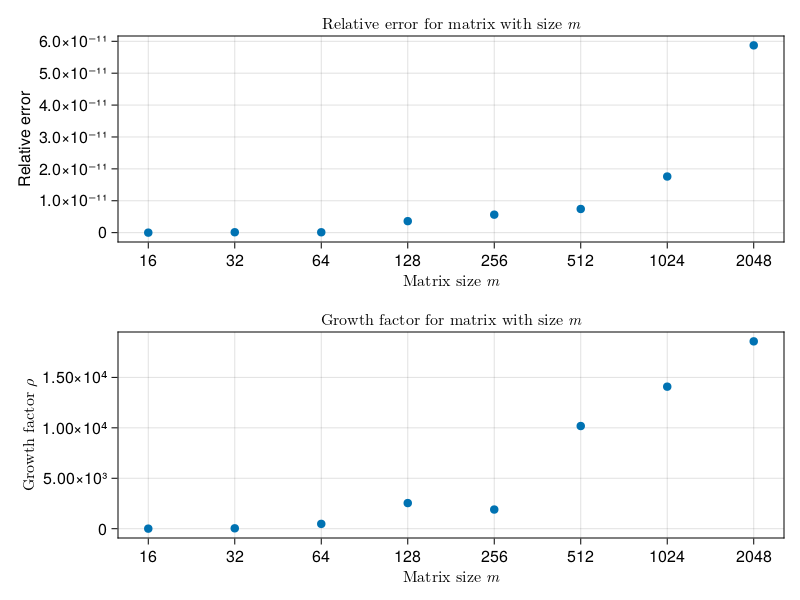
\includegraphics[width=120mm]{HW3_code/rel_error_and_growth_no_pivot.png}
  \end{center}
  \caption{Relative errors and growth factors, without pivoting}
  \label{fig:figure1}
\end{figure}

\quad See Fig. 1.
The floating point type used by my program is \verb|Float64|.
All tested matrices are normally distributed with a mean of $0$ and a standard deviation of $1$, with a unit diagonal offset (to help unpivoted factorization not get stuck), and no row permutations.
Relative error was computed as
$$\dfrac{\|\tilde{\vct{b}}-\vct{b}\|_2}{\|\vct{b}\|_2}.$$

\subsection*{(d) [5 pts]}
Go to section (d) of the file \texttt{HW3\_your\_code.jl} and implement the unpivoted LU factorization. 
Your code should pass the assertions in section (c) of \texttt{HW3\_driver.jl}.
Your function should take the matrix $A$ as an input to modify in place, and return an integer array $P$ according to the specifications of (a).
Repeat the experiment of (c) using the pivoted LU factorization. 

\begin{figure}[htb]
  \begin{center}
  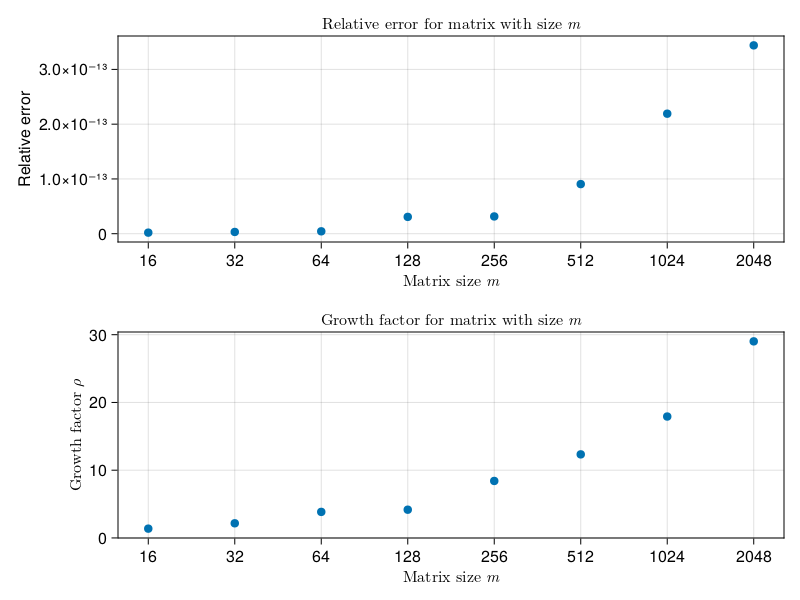
\includegraphics[width=120mm]{HW3_code/rel_error_and_growth_pivot.png}
  \end{center}
  \caption{Relative errors and growth factors, with pivoting}
  \label{fig:figure2}
\end{figure}

\quad See Fig. 2.
Note that, as expected, row pivoting results in a dramatic reduction in the growth factor, bringing it down from a max of $\approx2\cdot10^4$ to a max of $\approx 30$!
Also, the relative errors are consistently reduced by 2-4 decimal places (varying across experiments).

\textit{Note that the two experiements were run with different random matrices,} so we can't make an exact 1:1 comparison.

\subsection*{(e) [5 pts]}
Go to section (e) of the file \texttt{HW3\_driver.jl} and implement a function that takes an integer $m$ as an input and returns an $m \times m$ matrix as introduced in problem 2 (d).
Plot the error of the solution when solving equations in this matrix as a function of $m$. 
Compare the error to the built-in solution (the $\backslash$ operator). 
Draw your conclusions from this comparison. 

\begin{figure}[htb]
  \begin{center}
  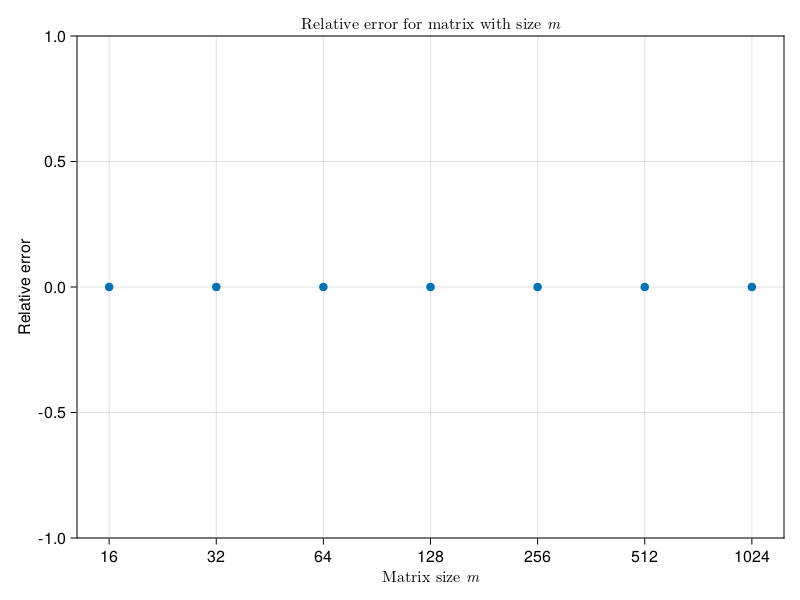
\includegraphics[width=120mm]{HW3_code/rel_error_and_growth_no_pivot_gm.png}
  \end{center}
  \caption{Relative errors and growth factors, with pivoting\\Using growth matrix}
  \label{fig:figure3}
\end{figure}

\quad See Fig. 3.
For this special kind of maximum-growth matrix, we can see that there is \textit{no difference} between our solution and the built-in $\backslash$ operator.

When I print out the resulting $LU$ factorization, the results look exactly accurate, so I have convinced myself this is not an error.
I suppose this results in part from all numbers in the input matrix and the $LU$ matrices being represented exactly by floating point representations of natural numbers.
Beyond this, I am not sure, and I look forward to learning more about this phenomenon!
(I have a feeling there's a simple explanation I'm missing...)

\bibliography{refs}

\end{document}
